% =============================================================================
\bloco{1}{Price indices, new goods, welfare and growth accounting}{Kurlat chs.~1--2, 5 \,\textbullet\, 25 points}

\questao{(10 points) Objective items.}

\textbf{a)} (3 points) A household with CES preferences (elasticity of substitution $\eta>0$, $\eta\neq1$) over two goods spends a
share $\omega\in(0,1)$ of its budget on good 1 and $1-\omega$ on good 2 at base prices. The price of good 1 is multiplied by $R>1$; the
price of good 2 does not change. The log overstatement of the true change in the cost of living by the Laspeyres index $L$,
$\ln(L/P^*)$ with $P^*$ the exact index, is:
\begin{alternativas}
\item $\ln(\omega R+1-\omega)-\omega\ln R$
\item $\ln(\omega R+1-\omega)-\frac{1}{\eta-1}\ln(\omega R^{\eta-1}+1-\omega)$
\item $\ln(\omega R+1-\omega)-\frac{1}{1-\eta}\ln(\omega R^{1-\eta}+1-\omega)$
\item $\ln(\omega R+1-\omega)-\ln(\omega R^{\eta-1}+1-\omega)$
\end{alternativas}
\gabarito{C}
\begin{sol}
\passo{exact index}{Under CES the cost of a util is $P=\big(\sum_i(p_i/b_i)^{1-\eta}\big)^{1/(1-\eta)}$ (Question 2(a); any $\eta>0$, $\eta\neq1$),
with base shares $w_i^0=(p_{i0}/b_i)^{1-\eta}/P_0^{1-\eta}$; so $P^*=\big(\sum_iw_i^0R_i^{1-\eta}\big)^{1/(1-\eta)}=(\omega R^{1-\eta}+1-\omega)^{1/(1-\eta)}$, the
power mean of order $1-\eta$ of $(R,1)$ with weights $(\omega,1-\omega)$.}
\passo{bias}{$L=\sum_iw_i^0R_i=\omega R+1-\omega$ is the power mean of order 1; logs give C. Power means rise with the order (Question 2(b))
and $1-\eta<1$, so the bias is positive and rises with $\eta$; it tends to 0 as $\eta\to0$ (Leontief: Laspeyres is exact), and to second
order in $\ln R$ it equals $(\eta/2)\operatorname{Var}(\ln R_i)=(\eta/2)\,\omega(1-\omega)(\ln R)^2$.}
\passo{distractors}{A is the Cobb--Douglas index (the limit $\eta\to1$) used for every $\eta$; B uses order $\eta-1$, the current-weight
formula of Question 2(b), with base weights; D makes two mistakes: order $\eta-1$ with base weights, as B, and no root $1/(\eta-1)$.}
\refbib{Kurlat (2020), ch.~1, \S1.2 (base-year versus final-year prices); Jones (2020), ch.~2, \S2.3.}
\end{sol}

\medskip
\textbf{b)} (3 points) \emph{Welfare $\times$ growth.} Over $T$ years Brazil's mean consumption grows at $g$ log points a year (initial
mean one), the variance of log consumption (normal) goes from $v_0$ to $v_T$, and the survival probability of Kurlat's single-year
experiment (life expectancy over 100) rises from $a_0$ to $a_T>a_0$; leisure is constant (absorbed into $\bar u$). Utility is
Kurlat--Jones--Klenow with $\sigma=1$ and positive flow utility at both dates. If $\lambda$ scales all date-0 consumption so that Rawls
is indifferent between date-0 and date-$T$ Brazil, the average annual growth of consumption-equivalent welfare, $(\ln\lambda)/T$, is:
\begin{alternativas}
\item $g+\frac{v_0-v_T}{2T}+\frac{1}{T}\big(\frac{a_T}{a_0}-1\big)\big(\bar u+gT-\frac{v_T}{2}\big)$
\item $g+\frac{v_T-v_0}{2T}+\frac{1}{T}\big(\frac{a_T}{a_0}-1\big)\big(\bar u+gT+\frac{v_T}{2}\big)$
\item $g+\frac{v_0-v_T}{2T}+\frac{1}{T}\ln\frac{a_T}{a_0}$
\item $g+\frac{v_T-v_0}{2T}+\frac{1}{T}\big(1-\frac{a_0}{a_T}\big)\big(\bar u+\frac{v_0}{2}\big)$
\end{alternativas}
\gabarito{A}
\begin{sol}
\passo{expected utility}{With $\sigma=1$ a living person gets $\bar u+\ln c$; survival is independent of consumption, so Kurlat's (2.2.1) gives
$\mathbb E[u]=a(\bar u+\mathbb E\ln c)$. If $\ln c\sim N(\mu,v)$, mean consumption is $e^{\mu+v/2}$, so $\mathbb E\ln c=\ln\bar c-v/2$:
$\mathbb E\ln c_0=-v_0/2$ and $\mathbb E\ln c_T=gT-v_T/2$.}
\passo{indifference}{(2.2.2) with date 0 as the reference, $a_0(\bar u+\ln\lambda-v_0/2)=a_T(\bar u+gT-v_T/2)$, gives
$\ln\lambda=(a_T/a_0)(\bar u+gT-v_T/2)-\bar u+v_0/2$. Adding and subtracting $\bar u+gT-v_T/2$ splits it into consumption, $gT$;
inequality, $(v_0-v_T)/2$; and longevity, $(a_T/a_0-1)(\bar u+gT-v_T/2)>0$. Dividing by $T$ gives A.}
\passo{distractors}{B uses $\mathbb E\ln c=\ln\bar c+v/2$; C treats longevity as a proportional consumption gain, ignoring that a year is
worth its flow utility; D makes two mistakes: it takes date $T$ as the reference (scales date-$T$ consumption), weighting date-0 flow
utility by $1-a_0/a_T$, and uses $\mathbb E\ln c=\ln\bar c+v/2$, as B does.}
\refbib{Kurlat (2020), ch.~2, \S2.2, eqs.\ (2.2.1)--(2.2.2) and ``The Value of Life Expectancy''.}
\end{sol}

\medskip
\textbf{c)} (2 points, T or F) A Paasche price index can never exceed the corresponding Laspeyres index.
\gabarito{F}
\begin{sol}
\passo{Bortkiewicz decomposition}{With base expenditure weights $w_i$, price relatives $R_i^p=p_{i1}/p_{i0}$ and quantity relatives
$R_i^q=q_{i1}/q_{i0}$: $L=\sum_iw_iR_i^p\equiv\bar R^p$ and Paasche $=\sum_ip_{i1}q_{i1}/\sum_ip_{i0}q_{i1}=\sum_iw_iR_i^pR_i^q/\sum_iw_iR_i^q$, so
Paasche$/L=1+\operatorname{Cov}_w(R^p,R^q)/(\bar R^p\bar R^q)$, with $\bar R^q\equiv\sum_iw_iR_i^q$.}
\passo{counterexample}{Two goods, $w=(\frac12,\frac12)$, $R^p=(R,1)$ and $R^q=(Q,1)$ with $R,Q>1$ (demand shifts toward the good whose
price rises): $\operatorname{Cov}_w=(R-1)(Q-1)/4>0$ and Paasche$/L=1+(R-1)(Q-1)/[(R+1)(Q+1)]>1$. With stable CES preferences
Question 2(b) gives Paasche $\le P_1/P_0\le$ Laspeyres; the statement fails once tastes or qualities shift.}
\refbib{Kurlat (2020), ch.~1, \S1.2; Jones (2020), ch.~2, \S2.3.}
\end{sol}

\medskip
\textbf{d)} (2 points, T or F) \emph{PPP $\times$ productivity growth.} In Brazil and in the US labor is the only input and moves freely
between tradables and non-tradables (linear technologies); consumers buy a Cobb--Douglas basket with the same non-tradable share
$\gamma\in(0,1)$; tradables obey the law of one price; the exchange rate is constant. If Brazil's tradable productivity grows faster
than the US's while non-tradable productivity grows equally in both, Brazil's price level relative to the US's rises, at a rate that
increases with $\gamma$ and would be zero if all goods were tradable.
\gabarito{T}
\begin{sol}
\passo{within a country}{With $y_j=A_jL_j$, competition and one wage, $w=p_TA_T=p_NA_N$, so $p_N/p_T=A_T/A_N$. The unit cost of the
basket is $P=\kappa_\gamma p_T^{1-\gamma}p_N^{\gamma}=\kappa_\gamma p_T(A_T/A_N)^{\gamma}$, with $\kappa_\gamma=(1-\gamma)^{\gamma-1}\gamma^{-\gamma}$.}
\passo{across countries}{With $p_T^{BR}=Ep_T^{US}$, $P^{BR}/(EP^{US})=\big[(A_T^{BR}/A_N^{BR})/(A_T^{US}/A_N^{US})\big]^{\gamma}$, which grows at
$\gamma\big[(g_T^{BR}-g_T^{US})-(g_N^{BR}-g_N^{US})\big]=\gamma\Delta$, $\Delta\equiv g_T^{BR}-g_T^{US}>0$: positive, increasing in $\gamma$ and zero at $\gamma=0$:
non-tradables get dearer, with weight $\gamma$.}
\refbib{Kurlat (2020), ch.~1, \S1.2 (PPP comparisons); Romer (2012), ch.~4, \S4.2 (Balassa--Samuelson effect).}
\end{sol}

% -----------------------------------------------------------------------------
\questao{(15 points) Discursive. \emph{Measurement $\times$ growth accounting.} Consumers have CES preferences over
the set $\Omega_t$ of varieties available at date $t$,
\[U=\Big(\sum_{i\in\Omega_t}(b_ix_i)^{\frac{\eta-1}{\eta}}\Big)^{\frac{\eta}{\eta-1}},\qquad\eta>1,\]
where $b_i>0$ is a quality weight. The statistical agency (IBGE) observes prices and expenditure shares and builds its
deflators from varieties present in both periods. Growth rates are in log points per period.}

\textbf{a)} (3 points) Find the minimum expenditure needed to obtain one unit of utility at prices $p$, and each variety's
expenditure share.
\resolespaco
\begin{sol}
\passo{problem}{$\min\sum_ip_ix_i$ s.t.\ $\sum_i(b_ix_i)^{\rho}=1$, $\rho\equiv(\eta-1)/\eta\in(0,1)$. $U$ is concave and homogeneous of degree one,
so the upper contour set is convex and the first-order conditions give the minimum: $p_i=\mu\rho b_i^{\rho}x_i^{\rho-1}$, $\mu$ the multiplier.}
\passo{demands}{$x_i=(\mu\rho)^{\eta}b_i^{\eta-1}p_i^{-\eta}$, using $1/(1-\rho)=\eta$ and $\rho/(1-\rho)=\eta-1$. The constraint gives
$(\mu\rho)^{\eta-1}\sum_i(p_i/b_i)^{1-\eta}=1$.}
\passo{cost of a util}{Spending $=(\mu\rho)^{\eta}\sum_ib_i^{\eta-1}p_i^{1-\eta}=(\mu\rho)^{\eta}(\mu\rho)^{1-\eta}=\mu\rho$, so
\[P=\Big(\sum_i(p_i/b_i)^{1-\eta}\Big)^{\frac1{1-\eta}},\qquad w_i=\frac{p_ix_i}{P}=\frac{(p_i/b_i)^{1-\eta}}{P^{1-\eta}}.\]
By homotheticity $P$ does not depend on utility: it is a true price index, and $\mu\rho=P$ is the marginal cost of a util.}
\intuicao{Only quality-adjusted prices $p_i/b_i$ matter; shares fall with them, faster the larger $\eta$.}
\refbib{Kurlat (2020), ch.~1, \S1.2 (substitution, quality and new-goods biases).}
\rubrica{
\item FOC and demands: 1.5 pts; $P$ and the shares: 1.5 pts. Formula quoted without derivation: max.\ 1 pt in the item.
}
\end{sol}

\textbf{b)} (3 points) Keep the set of varieties fixed between dates 0 and 1. Express the exact index $P_1/P_0$ in terms of
observable price relatives $R_i=p_{i1}/p_{i0}$ and shares, rank it against the Laspeyres and Paasche indices, and approximate the
Laspeyres bias to second order in the dispersion of $\ln R_i$.
\resolespaco
\begin{sol}
\passo{base and current weights}{By (a), $(P_1/P_0)^{1-\eta}=\sum_i(p_{i1}/b_i)^{1-\eta}/P_0^{1-\eta}=\sum_iw_i^0R_i^{1-\eta}$, so $P_1/P_0=M_{1-\eta}(R;w^0)$, where
$M_r(R;w)\equiv\big(\sum_iw_iR_i^r\big)^{1/r}$ is the power mean of order $r$. Since $w_i^1=w_i^0R_i^{1-\eta}/\sum_jw_j^0R_j^{1-\eta}$,
$\sum_iw_i^1R_i^{\eta-1}=1/\sum_jw_j^0R_j^{1-\eta}$, and $P_1/P_0=M_{\eta-1}(R;w^1)$.}
\passo{ranking}{Power means rise with the order: $d\ln M_r/dr=r^{-2}\sum_i\tilde w_i\ln(\tilde w_i/w_i)\ge0$ with $\tilde w_i\equiv w_iR_i^r/\sum_jw_jR_j^r$,
a Kullback--Leibler divergence, zero iff all $R_i$ are equal. Laspeyres $=\sum_iw_i^0R_i=M_1(R;w^0)$ and Paasche $=\big(\sum_iw_i^1/R_i\big)^{-1}=M_{-1}(R;w^1)$;
since $1-\eta<1$ and $\eta-1>-1$, Paasche $\le P_1/P_0\le$ Laspeyres, with equality iff all $R_i$ are equal.}
\passo{second order}{With $z_i=\ln R_i$, mean $\bar z$ and variance $V$ under $w^0$: $\sum_iw_i^0e^{rz_i}=e^{r\bar z}{\big(1+r^2V/2+O(|z-\bar z|^3)\big)}$,
so $\ln M_r=\bar z+rV/2+O(|z-\bar z|^3)$. Hence $\ln L-\ln(P_1/P_0)\approx V/2-(1-\eta)V/2=\eta V/2$.}
\intuicao{Laspeyres ignores substitution away from goods that became dearer; the gap grows with $\eta$ and with price dispersion.}
\refbib{Kurlat (2020), ch.~1, \S1.2; Jones (2020), ch.~2, \S2.3.}
\rubrica{
\item Exact index, both weightings: 1.5 pts; ranking proved: 1 pt (asserted: 0 for this line); second-order bias: 0.5 pt. Special
case (two goods, a given $\eta$) used for the general one: max.\ 1.5 pts.
}
\end{sol}

\textbf{c)} (3 points) Now some varieties are new at date 1 and none disappears. Find the exact index in terms of the index over
continuing varieties and observable shares. What happens as $\eta\to\infty$ and as $\eta\to1$?
\resolespaco
\begin{sol}
\passo{split the index}{Let $\mathcal C$ be the continuing set, $P_t^{\mathcal C}$ the index of (a) computed over $\mathcal C$ only, and
$\lambda_t\equiv\sum_{i\in\mathcal C}(p_{it}/b_i)^{1-\eta}/\sum_{i\in\Omega_t}(p_{it}/b_i)^{1-\eta}$, which by (a) is the expenditure share of continuing varieties at
$t$ ($\lambda_0=1$). Then $P_t^{1-\eta}=(P_t^{\mathcal C})^{1-\eta}/\lambda_t$.}
\passo{formula}{Raising to $1/(1-\eta)$: $P_t=P_t^{\mathcal C}\lambda_t^{1/(\eta-1)}$, so $P_1/P_0=(P_1^{\mathcal C}/P_0^{\mathcal C})\,(\lambda_1/\lambda_0)^{1/(\eta-1)}$, which needs only
shares, not the qualities $b_i$ of the new varieties.}
\passo{limits}{With $\lambda_1<1$ the log of the correction is $\ln\lambda_1/(\eta-1)<0$. It tends to $0$ as $\eta\to\infty$ (perfect substitutes add
nothing beyond their price) and to $-\infty$ as $\eta\to1^+$, so $P_1/P_0\to0$: new varieties become infinitely valuable.}
\intuicao{New varieties raise what a unit of spending buys; their share reveals by how much, and $\eta$ turns it into a price.}
\refbib{Kurlat (2020), ch.~1, \S1.2 (new-goods bias).}
\rubrica{
\item $\lambda_t$ as an observable share: 1 pt; formula derived: 1.5 pts; both limits, argued: 0.5 pt (asserted: 0 for this line).
}
\end{sol}

\textbf{d)} (3 points) The agency measures the continuing-variety consumption index exactly. New varieties appear only among
consumption goods, take a share $\nu\in(0,1)$ of date-1 consumption spending, and none disappears. Investment goods (nominal GDP
share $s_I\in(0,1)$, $s_C=1-s_I$) have their own deflator bias $\beta_I\in[0,g_K+\delta)$ from unmeasured quality change ($g_K$: true capital
growth; $\delta>0$: depreciation); labor and the capital share $\alpha\in(0,1)$ are measured correctly. On a balanced growth path, find
the consumption-deflator bias $\beta_C$, show that measured capital growth converges and at what speed, and find the distortion
$\Delta\equiv g_A^m-g_A$ of the measured Solow residual; compare $\beta_I=0$ with $\beta_I=\beta_C$.
\resolespaco
\begin{sol}
\passo{consumption bias}{By (c) with $\lambda_0=1$ and $\lambda_1=1-\nu$, true inflation is $\ln(P_1/P_0)=\ln(P_1^{\mathcal C}/P_0^{\mathcal C})+\ln(1-\nu)/(\eta-1)$, so the
measured deflator overstates it by $\beta_C=-\ln(1-\nu)/(\eta-1)>0$.}
\passo{measured output}{Real GDP growth is the share-weighted growth of its components, each equal to nominal growth minus its
deflator: $g_Y^m=s_C(g_C-\beta_C)+s_I(g_I-\beta_I)=g_Y-(s_C\beta_C+s_I\beta_I)$.}
\passo{measured capital}{Perpetual inventory (continuous time): $\dot K^m=I^m-\delta K^m$, with $I^m$ growing at $g_K-\beta_I$ on the balanced path,
so $x\equiv K^m/I^m$ obeys $\dot x=1-(g_K-\beta_I+\delta)x$. As $g_K-\beta_I+\delta>0$, $x$ converges monotonically to $1/(g_K-\beta_I+\delta)$ at that rate
(half-life $\ln2/(g_K-\beta_I+\delta)$), and $\dot K^m/K^m=1/x-\delta\to g_K-\beta_I$: understated by $\beta_I$.}
\passo{residual}{By Kurlat's (5.4.2), $g_A^m=g_Y^m-\alpha g_K^m-(1-\alpha)g_L$ and $g_A=g_Y-\alpha g_K-(1-\alpha)g_L$, so
\[\Delta\equiv g_A^m-g_A=-(s_C\beta_C+s_I\beta_I)+\alpha\beta_I=-s_C\beta_C-(s_I-\alpha)\beta_I.\]}
\passo{two cases}{$\beta_I=0$: $\Delta=-s_C\beta_C$. $\beta_I=\beta_C$: $\Delta=-(1-\alpha)\beta_C$, using $s_C+s_I=1$. Both are negative, and
$\Delta(\beta_C)-\Delta(0)=(\alpha-s_I)\beta_C$: the uniform bias distorts less iff $\alpha>s_I$.}
\intuicao{Understated output lowers measured TFP growth and understated capital raises it; equipment quality change is embodied
technical progress (Romer's problem 1.12), booked as TFP.}
\refbib{Kurlat (2020), ch.~5, \S5.4, eq.\ (5.4.2); Romer (2012), ch.~1, \S1.7 and problem 1.12.}
\rubrica{
\item $\beta_C$: 0.5 pt; output bias: 0.5 pt; capital (convergence, speed, bias $\beta_I$): 1 pt, convergence asserted: 0 for this line;
residual and the two cases: 1 pt. Caps: capital channel ignored: max.\ 1.5 pts; $\beta_I=\beta_C$ used as the general case: max.\ 1.5 pts.
}
\end{sol}

\textbf{e)} (3 points) \emph{Parameter analysis.} How do $\beta_C$ and $\Delta$ depend on $\eta$, $\nu$, $\beta_I$, $\alpha$ and $s_I$? Prove and tabulate
the signs. Find the $\beta_I^*$ at which $\Delta$ changes sign, when it exists, and how it moves with the parameters. Give the limits
of $\beta_C$ as $\eta\to1^+$, $\eta\to\infty$ and $\nu\to0$, and draw $\beta_C$ against $\eta$ for three new-variety shares $\nu_1<\nu_2<\nu_3$.
\resolespaco
\begin{sol}
\passo{signs of $\beta_C$}{From $\beta_C=\ell/(\eta-1)$ with $\ell\equiv-\ln(1-\nu)>0$: $\partial_\eta\beta_C=-\ell/(\eta-1)^2<0$, $\partial_\nu\beta_C=1/[(1-\nu)(\eta-1)]>0$
and $\partial_\eta^2\beta_C=2\ell/(\eta-1)^3>0$; $\beta_C$ does not depend on $\beta_I$, $\alpha$ or $s_I$.}
\passo{signs of $\Delta$}{From $\Delta=-(1-s_I)\beta_C-(s_I-\alpha)\beta_I$: $\partial_\eta\Delta=-(1-s_I)\partial_\eta\beta_C>0$, $\partial_\nu\Delta=-(1-s_I)\partial_\nu\beta_C<0$,
$\partial_{\beta_I}\Delta=\alpha-s_I$, $\partial_\alpha\Delta=\beta_I\ge0$ and $\partial_{s_I}\Delta=\beta_C-\beta_I$.}
\passo{sign switch}{$\Delta$ is affine in $\beta_I$ with intercept $-s_C\beta_C<0$. If $\alpha>s_I$ it has the unique root $\beta_I^*=s_C\beta_C/(\alpha-s_I)>0$, and
$\Delta>0$ iff $\beta_I>\beta_I^*$ (admissible only if $\beta_I^*<g_K+\delta$); if $\alpha\le s_I$, $\Delta<0$ for every $\beta_I\ge0$. Moreover
$\partial_\alpha\beta_I^*=-s_C\beta_C/(\alpha-s_I)^2<0$, $\partial_{s_I}\beta_I^*=(1-\alpha)\beta_C/(\alpha-s_I)^2>0$, and $\beta_I^*\propto\beta_C$ inherits the signs of $\beta_C$ in $\eta$
and $\nu$. Table: an expression stands for its sign; row $\beta_I^*$ assumes $\alpha>s_I$.}
\begin{center}
\begin{minipage}[c]{0.44\linewidth}\centering\small
\begin{tabular}{lccccc}
\toprule
 & $\eta$ & $\nu$ & $\beta_I$ & $\alpha$ & $s_I$ \\
\midrule
$\beta_C$ & $-$ & $+$ & $0$ & $0$ & $0$ \\
$\Delta$ & $+$ & $-$ & $\alpha-s_I$ & $\beta_I$ & $\beta_C-\beta_I$ \\
$\beta_I^*$ & $-$ & $+$ & $0$ & $-$ & $+$ \\
\bottomrule
\end{tabular}
\end{minipage}\hfill
\begin{minipage}[c]{0.54\linewidth}\centering
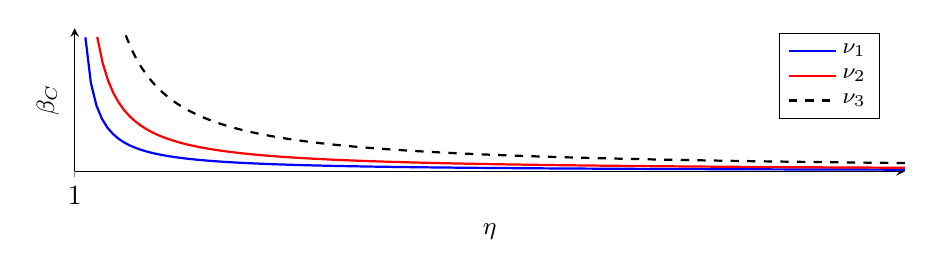
\begin{tikzpicture}
\begin{axis}[width=\linewidth,height=3.4cm,xmin=1,xmax=8,ymin=0,ymax=1.25,axis lines=left,xtick={1},xticklabels={$1$},
  ytick=\empty,xlabel={$\eta$},ylabel={$\beta_C$},legend style={font=\footnotesize},legend pos=north east,label style={font=\small}]
\addplot[thick,blue,domain=1.09:8,samples=150]{-ln(0.9)/(x-1)};
\addplot[thick,red,domain=1.19:8,samples=150]{-ln(0.8)/(x-1)};
\addplot[thick,black,dashed,domain=1.43:8,samples=150]{-ln(0.6)/(x-1)};
\legend{$\nu_1$,$\nu_2$,$\nu_3$}
\end{axis}
\end{tikzpicture}
\end{minipage}
\end{center}
\passo{limits and reading}{$\beta_C\to\infty$ as $\eta\to1^+$ (new varieties become essential), $\beta_C\to0$ as $\eta\to\infty$, and $\beta_C=\nu/(\eta-1)+O(\nu^2)\to0$
as $\nu\to0$: the curves fall, are convex, ordered by $\nu$, asymptotic to $\eta=1$ and to the axis. Knife-edge $\alpha=s_I$: $\Delta=-s_C\beta_C$ for all
$\beta_I$, and $\beta_I^*\to\infty$ as $\alpha\downarrow s_I$. Reading: on a one-good balanced path $I=(g_K+\delta)K$ and $\alpha=f'(k)K/Y$, so
$\alpha-s_I=(K/Y)\big(f'(k)-\delta-g_K\big)$: $\alpha>s_I$ iff capital is below the golden rule (Kurlat (4.3.4)), the dynamically efficient case,
where faster equipment quality change shrinks the TFP understatement and reverses it above $\beta_I^*$. The consumption bias
is large for differentiated goods with many new varieties, not for commodities.}
\refbib{Kurlat (2020), ch.~1, \S1.2; ch.~4, \S4.3, eq.\ (4.3.4) (golden rule); ch.~5, \S5.4.}
\rubrica{
\item Signs proved: 1 pt; table: 0.5 pt; $\beta_I^*$ (condition, signs): 0.5 pt; limits and reading: 0.5 pt (a limit asserted: 0 for this
line); signs without proof or reading: max.\ 1.5 pts. Graph, scored separately: labeled axes, three decreasing convex curves
ordered by $\nu$, asymptote $\eta=1$: 0.5 pt.
}
\end{sol}
